\documentclass[a4paper,twoside]{report} % for a report (default)

\usepackage{amsmath}
\usepackage{bftn} % You need this
\usepackage{cite}
\usepackage{color}
\usepackage{listings}
\usepackage{xspace}

\title{Porting Barrelfish to TilePro} % title of report
\author{Robert Radkiewicz, Xiaowen Wang} % author
\tnnumber{017} % give the number of the tech report
\tnkey{TilePro Porting} % Short title, will appear in footer

% \date{Month Year} % Not needed - will be taken from version history

% Source: http://www.martin-demling.de/2011/06/memory-maps-in-latex-using-the-bytefield-package/
% Needs bytefield package in at least version 2.0, but the compiled version should be shipped next to this document.
\usepackage{bytefield}

% facilitates the creation of memory maps. Start address at the bottom, end address at the top.
% syntax: \memsection{end address}{start address}{height in lines}{text in box}
\newcommand{\memsection}[4]{
\bytefieldsetup{bitheight=#3\baselineskip} % define the height of the memsection
\bitbox[]{10}{
\texttt{#1} % print end address
\\ \vspace{#3\baselineskip} \vspace{-1\baselineskip} \vspace{-#3pt} % do some spacing
\texttt{#2} % print start address
}
\bitbox{20}{#4} % print box with caption
}

%%%%%%%%%%%%%%%%%%%%%%%%%%%%%%%%%%%%%%%%%%%%%%%%%%%%%%%%%%%%%%%%%%%%%%%%%%%%%

\begin{document}
\maketitle

%
% Include version history first
%
\begin{versionhistory}
\vhEntry{0.0}{22.02.2013}{rrad}{Initial version}
\end{versionhistory}

% \intro{Abstract}		% Insert abstract here
% \intro{Acknowledgements}	% Uncomment (if needed) for acknowledgements
% \tableofcontents		% Uncomment (if needed) for final draft
% \listoffigures		% Uncomment (if needed) for final draft
% \listoftables			% Uncomment (if needed) for final draft

\lstset{
  language=C,
  basicstyle=\ttfamily \small,
  flexiblecolumns=false,
  basewidth={0.5em,0.45em},
  boxpos=t,
}

\newcommand{\note}[1]{[\textcolor{red}{\emph{#1}}]}
\newcommand{\Intf}{\texttt{/kernel/include/serial.h}\xspace}

\tableofcontents

%%%%%%%%%%%%%%%%%%%%%%%%%%%%%%%%%%%%%%%%
% chapter of introduction
%%%%%%%%%%%%%%%%%%%%%%%%%%%%%%%%%%%%%%%%
\chapter{Introduction}

The project mainly investigates how to port Barrelfish onto TilePro architecture and make use of TilePro network structure to implement core-to-core communication instead of a shared-memory mechanism provided originally in Barrelfish. The whole porting process involves some general configurations of image booting, virtual memory system, context switch, interrupts and system calls, inter-dispatcher communication and so on. So far Barrelfish can completely boots up on two cores at least, while the inter-core communication between them is ongoing using TilePro user dynamic network. Moreover, some user applications could be executed on these running cores correctly.

\section{HOWTO}
Only the differences to other portings are described below:

\begin{itemize}
  \item After checking out change to the `tile\_on\_bf' branch with `hg update tile\_on\_bf'.
  \item Have the Tilera MDE installed.
  \item Setup the environment variable `\$TILERA\_ROOT' with the help of the `bin/tile-env' script from the MDE.
  \item You should be able to use `tile-cc' from the command line now.
  \item Use the script `tools/tilepro/createTileImportsDir.sh' to create a directory with some links to TilePro .h-files.
  \item Setup the environment variable `\$TILE\_IMPORTS', which points to that directory.
\end{itemize}

\section{Known Limitations}
\begin{itemize}
  \item Cannot print reliably 64bit values, workaround is to print upper and lower 32bit. (Maybe an error in the newlib? Barrelfish uses a release from 2011, TilePro shipped a release from 2004 plus the tile machine part, which is merged manually.) Does not happen in simply cases, maybe only if the value is read from the stack?
  \item No timer yet, everything runs do to non-preemtive behavior. Timer code stub is available.
  \item Other architectures cannot be compiled with the same code basis, as the first two values in the file `capabilities/caps.hl' (`cte\_size' \& `dispatcher\_size') are different and cannot be defined in a platform-dependent way.
  \item getc() is not implemented.
\end{itemize}

\section{Port to Tile-Gx}
It is not expected to run on the Tile-Gx platform. The virtual address space of the Tile-Gx is 64bits instead of 32bits, that's one of the reasons. To have an idea about what need to be changed run
\begin{verbatim}
  find -name "*.[chS]" | xargs grep "#ifdef __tilegx__"
\end{verbatim}
and
\begin{verbatim}
  find -name "*.[chS]" | xargs grep "#if CHIP_VA_WIDTH"
\end{verbatim}
inside the `src/sys/bogux' folder of the MDE and inside the `arch/tile' folder of a Linux release (version 3.6 or higher?).

%*****************************************
% Implementation chapter 
%*****************************************
\chapter{Implementation}

\section{Booting an OS on Tilera}
In this section we describe in detail how to generically boot up an operating system on the TilePro architecture.

\subsection{Shipping the Kernel}
Barrelfish intends to ship the kernel to the processor with the help of Multiboot Specification, which is a part of GRUB. There is no Multiboot-implementation for Tilera, so we use the Tilera toolset to boot the kernel instead. In this toolset the first booters (level 0.5 and level 1 boot loader), hypervisor, hypervisor configuration file and the kernel are bundled to a bootrom file, which can be sent to the hardware.

\begin{figure}
  \centering
  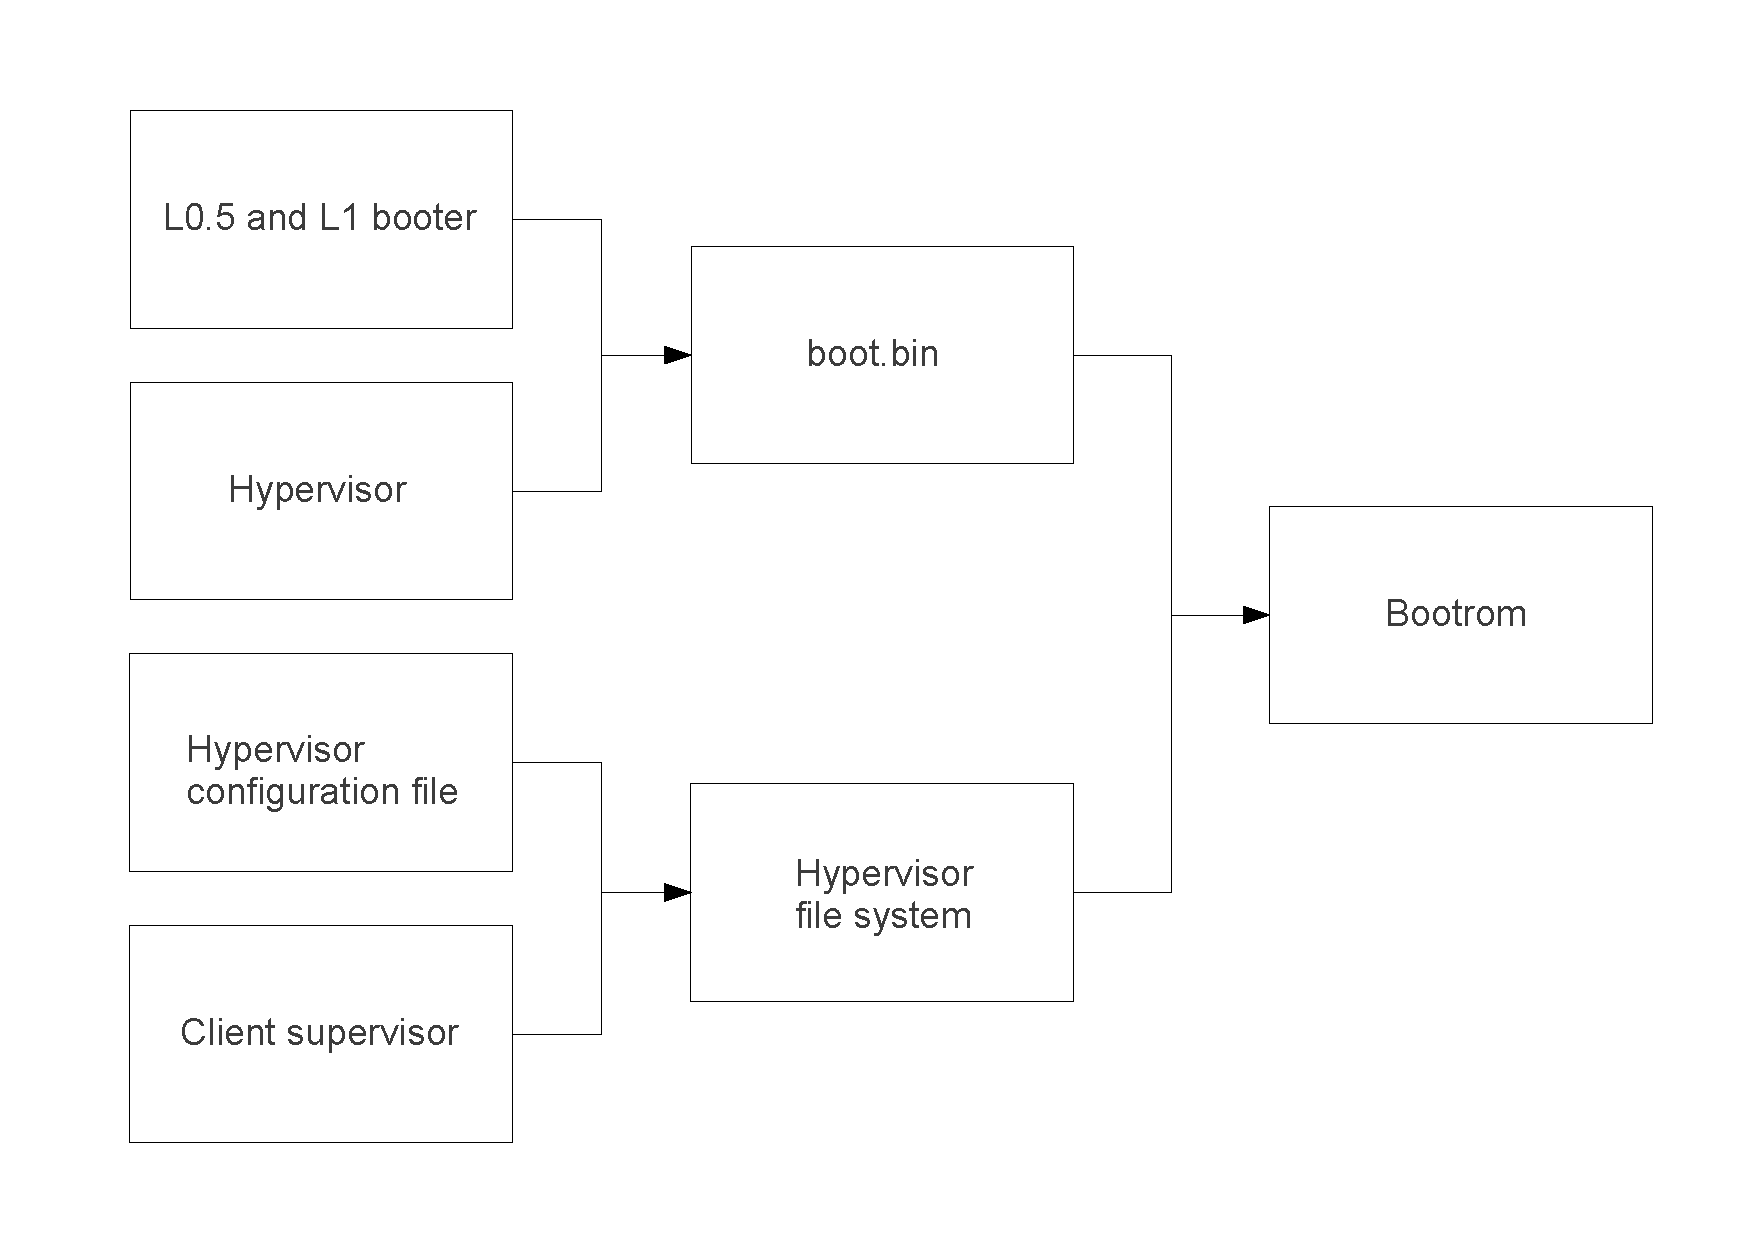
\includegraphics[scale=0.4]{figures/make_bootrom}
  \caption{Procedure to create a bootrom file}
  \label{pic:bootrom}
\end{figure}

\subsection{Hypervisor}
\label{sec:hypervisor}
The operating system can work either directly on the hardware or with a hypervisor in between. The mode to run directly on the hardware is called Bare Metal Environment. The hypervisor is a light layer, which is intended to help with the implementation of an OS on top of TilePro and make the porting to a future Tilera architecture easier. The hypervisor is designed to be very lightweight and is only running when explicitly called by the OS or if an interrupt occurs. This design makes the hypervisor a efficient tool without introducing any critical barriers during the porting process, therefore we decided to use it.

The hypervisor will get started when the bootrom is loaded on the architecture. It will load the kernel ELF file, put all segments into the specified physical addresses and jump to the entry point address to hand over control to the supervisor. The supervisor then has full control over the machine and can carry out its boot-up.

The hypervisor is not able to handle any relocations defined in the ELF file, because this is not needed for traditional operating systems, where all cores use the same kernel image. However in Barrelfish all kernels must be loaded to separate memory locations to be able to work on heterogeneous platforms, where different kernel images are needed. To be able to load the kernel image to different memory locations, we use a bootloader instead of the kernel. This bootloader is loaded by the hypervisor and maps the memory location for the data section depending on the core it is executed on. The real kernel is then loaded to this memory and executed. So the kernel is loaded to the same virtual address on each core, but to a different physical one. As an alternative to this, would be to let the bootloader perform some relocations on the kernel image.

\subsection{Overview of Booting Process}
The main steps of the booting process for the first core are listed below:
\begin{enumerate}
  \item Ship bundled hypervisor, bootloader, kernel \& program files;
  \item The hypervisor loads the bootloader ELF-file;
  \item Hypervisor sets the program counter to the entry point of the ELF-file;
  \item Install initial page table \& activate memory translation;
  \item Set up tile-specific kernel stack;
  \item Copy page table to a tile-specific location;
  \item Add tile-specific data section mapping;
  \item Switch to the new page table;
  \item Load kernel module and jump to its entry point;
  \item Slice the physical memory in sections, one for each core;
  \item Set up \emph{init}'s address space;
  \item Load ELF modules defined in menu.lst;
  \item Parse the given command line;
  \item Load \emph{init} module;
  \item A timer should be initialized at this moment;
  \item The hypervisor is told to start up all other cores;
  \item Context switch to \emph{init} in user mode;
  \item \emph{crt0} starts the runtime system, which starts bootstrap thread and initializes local message passing;
  \item \emph{init} starts \emph{monitor} \& \emph{mem{\textunderscore}serv}, and then exits;
  \item \emph{monitor} starts other modules;
  \item \emph{spawnd} initiates the second core;
  \item \emph{monitor} on the second core starts up;
  \item Two \emph{monitors} on different cores start remote inter-core communication, establishing a binding between two dispatchers.
\end{enumerate}

The booting process is somewhat different for all following cores:
\begin{enumerate}
  \item Hypervisor waits until the first core tells it to start the other cores;
  \item Hypervisor sets the program counter to the entry point of the ELF-file;
  \item Install initial page table \& activate memory translation;
  \item Set up tile-specific kernel stack;
  \item Copy page table to a tile-specific location;
  \item Add tile-specific data section mapping;
  \item Switch to the new page table;
  \item Load kernel module and jump to its entry point;
  \item Wait until the first core starts up this particular core;	
  \item Set up \emph{monitor}'s address space;
  \item Load \emph{monitor} module;
  \item A timer should be initialized at this moment;
  \item Context switch to \emph{monitor} in user mode;
  \item \emph{crt0} starts the runtime system, which starts bootstrap thread and initializes local message passing;
  \item \emph{monitor} starts remote inter-core communication with the first core by establishing a binding with corresponding dispatcher.
  \item \emph{spawnd} starts up.
\end{enumerate}

One interesting thing is here that the hypervisor only allows to start up all cores at once, but Barrelfish needs to start up one core at a time. To combine this different approaches, we are telling the hypervisor to start up all cores very early. Those cores then do some startup and wait for a special message. This message is send via the UDN network.

In contrast to other implementations of Barrelfish, on the TilePro platform some configurations have been already defined at compile time:
\begin{itemize}
  \item Most virtual address mappings are put into the data section of the kernel;
  \item The memory of the initial virtual mappings are allocated by the hypervisor while allocating the sections;
  \item For exception handling the interrupt vector is put into a special section, which is loaded to a well-known address.
\end{itemize}

In this boot process, no devices are initialized, because no devices are supported at the moment.

\section{newlib}
Barrelfish uses newlib as C standard library. A amount of functions inside Barrelfish are implemented with this particular C standard library, including introducing some crucial changes. This forces us to use the newlib. Newlib contains some machine-dependent files, which are implemented for a big number of systems. Unfortunately the official newlib release, which is used in Barrelfish, does not support TilePro platform. Tilera themselves give out a version of newlib as part of their distribution in order to support TilePro platform, but this distribution is based on a newlib released in 2004, so it could not be used as replacement for the existing newlib in Barrelfish. Then we have to merge some files manually according to the newlib FAQ, to get a working newlib both on Barrelfish and TilePro platform.

\section{Virtual Memory}
The memory layout is determined both by the platform and the OS. Barrelfish requires a large section, which is mapped 1:1 to the physical section, to be able to access physical addresses by a simple calculation (subtracting an offset). Furthermore it needs one part at the beginning, where the multiboot information for the other cores is lying. This 1:1 section must be handled as a special case for TilePro, because it has the property that the virtual address space is smaller than the physical address space (32-bit vs. 64-bit). With this property we are not able to maintain this mapping over the whole needed memory, if there is a lot of physical memory installed. So we have a mapping which is different from each core, by slicing the memory in core-wise. This scheme is working due to the property of Barrelfish not to share any memory between cores. TilePro only has some reserved addresses at the end of the virtual memory range, which are used by the hypervisor internally. There are no reserved physical addresses because an OS on top of the hypervisor only sees Client Physical Addresses, which are translated rapidly to real physical addresses by the hypervisor. This abstraction works in practice, so that we do not need to care about this translation and just handled the client physical addresses, as they would be real physical addresses.

The shipping process has some requirements on the memory layout in the sense that the information, which the kernel composes different sections (text, data, ...), must be told to the booter. This information is put into the ELF file via a linker script. The initial P=V mode (virtual address is mapped to the same physical address), which is active until the first page table has been installed, ensures that all needed virtual addresses are statically translated to physical addresses. As mentioned before in Section~\ref{sec:hypervisor} we need to map the data section of the kernel separately for each core. To be able to do so, we need a different initial page table for each core, differentiated by calculating the core ID. The stack for the kernel must be also different per core, but we just use different memory part next to each other, otherwise we would need to write the mappings without having a stack, i.e. in assembly. All these requirements lead us to create the virtual and physical memory layout shown in Figure \ref{pic:va} and Figure \ref{pic:pa} respectively.

%Virtual memory
\begin{figure}
\centering
\begin{bytefield}{24}
	\memsection{0xFFFF\ FFFF}{0xFE00\ 0000}{2}{-- hypervisor --}\\	
	\begin{rightwordgroup}{code section,\\one large page size}
		\memsection{}{0xFD03\ 0000}{1.5}{Kernel-Text}\\
		\memsection{}{0xFD02\ 0000}{1.5}{Bootloader-Text}\\
		\memsection{}{0xFD01\ 0000}{1.5}{Hypervisor glue}\\
		\memsection{}{0xFD00\ 0000}{1.5}{PL 1 Interrupt vectors}
	\end{rightwordgroup}\\
	\begin{rightwordgroup}{one large page size}
		\memsection{}{0xFC00\ 0000}{2}{Kernel stacks, 64k per tile}
	\end{rightwordgroup}\\
	\begin{rightwordgroup}{\textasciitilde 1.9~GB}
		\memsection{}{0x8000\ 0000}{4}{kernel space}
	\end{rightwordgroup}\\
	\begin{rightwordgroup}{\textasciitilde 2~GB}
		\memsection{}{0x0100\ 0000}{4}{user space}
	\end{rightwordgroup}\\
	\begin{rightwordgroup}{several small pages}
		\memsection{}{0x0000\ 0000}{2}{Barrelfish internal}
	\end{rightwordgroup}\\
\end{bytefield}
\caption{Virtual memory layout}
\label{pic:va}
\end{figure}

%Barrelfish internal, virtual memory
\begin{figure}
\centering
\begin{bytefield}{24}
	\begin{rightwordgroup}{1~MB}
		\memsection{0xFF\ 0000}{0xF0\ 0000}{2}{rodata + data, mapped per core}
	\end{rightwordgroup}\\
	\memsection{}{0xD0\ 0000}{1.5}{--unmapped--}\\
	\begin{rightwordgroup}{L1 + 1 * L2 for up to 256 cores}
		\memsection{}{0xC0\ 0000}{2}{page tables, sliced per core}
	\end{rightwordgroup}\\
	\memsection{}{0xB1\ 0000}{1.5}{--unmapped--}\\
	\begin{rightwordgroup}{size should be stable}
		\memsection{}{0xA0\ 0000}{2}{bootloader data}
	\end{rightwordgroup}\\
	\memsection{}{0x28\ 0000}{1.5}{--unmapped--}\\
	\begin{rightwordgroup}{Tell app cores their properties}
		\memsection{}{0x27\ 0000}{2}{multiboot data}
	\end{rightwordgroup}\\
	\begin{rightwordgroup}{mapped dynamically}
		\memsection{}{0x07\ 0000}{1.5}{DISPATCHER}\\
		\memsection{}{0x05\ 0000}{1.5}{BOOT\_ARGS}\\
		\memsection{}{0x01\ 0000}{1.5}{BOOT\_INFO}
	\end{rightwordgroup}\\
	\begin{rightwordgroup}{for NULL pointers}
		\memsection{}{0x00\ 0000}{1.5}{--unmapped--}
	\end{rightwordgroup}\\
\end{bytefield}
\caption{Barrelfish internal virtual memory layout}
\label{pic:bf_internel}
\end{figure} 

%Physical memory
\begin{figure}
\centering
\begin{bytefield}{24}
	\begin{rightwordgroup}{sliced per core}
		\memsection{}{0x1300\ 0000}{4}{Free space}
	\end{rightwordgroup}\\
	\begin{rightwordgroup}{mapped per core}
		\memsection{}{0x0300\ 0000}{3}{256 * (rodata + data)}
	\end{rightwordgroup}\\
	\begin{rightwordgroup}{statically mapped}
		\memsection{}{0x0200\ 0000}{2}{Kernel stacks, 64k per tile}\\
		\memsection{}{0x0100\ 0000}{2}{Barrelfish internal}\\
		\memsection{}{0x0003\ 0000}{1.5}{Kernel Text}\\
		\memsection{}{0x0002\ 0000}{1.5}{Bootloader Text}\\
		\memsection{}{0x0001\ 0000}{1.5}{Hypervisor glue}\\
		\memsection{}{0x0000\ 0000}{1.5}{PL 1 Interrupt vectors}
	\end{rightwordgroup}\\
\end{bytefield}
\caption{Physical memory layout}
\label{pic:pa}
\end{figure}

Figure \ref{pic:va} describes virtual memory layout. Some addresses are pre-determined by TilePro, e.g. addresses from 0xFD000000 to 0xFE00000 are for kernel code section, addresses above 0xFE000000 are for hypervisor, we cannot use these memory space for other purposes. A special part in Figure \ref{pic:va} is called Barrelfish internal, pictured in detail in Figure \ref{pic:bf_internel}. In this area, some Barrelfish-related data should be put here to specifically start up the first user-level process init in terms of Barrelfish convention. Furthermore, due to the fact that TilePro page size (64KB for small page and 16MB for large page) is normally much larger than other architectures', for instance, in x86 and ARM, small page size is 4KB, we decided to lay more data in this area, such as kernel data section, to save some memory space. For the physical memory, as shown in Figure \ref{pic:pa}, except those statically mapped parts where mainly contain kernel data, we have separate data section for each core, and the remaining free space is sliced per core, so that one core cannot interfere with others, and it is possible to support heterogeneous hardware.

\section{ASIDs}
TilePro supports the use of Address Space Identifiers (ASIDs) and we use them in order to avoid flushing the Translation Lookaside Buffer (TLB) during the context switch. Every dispatcher on one core will be assigned an unique ASID, then during the context switch, the TLB needs not to be flushed, since each process in the page table is recognizable by its ASID. However there is a limit of totally 256 ASIDs per core restricted by TilePro hardware and when this number is reached, it is not possible to spawn new dispatchers.

The kernel memory content has no ASID and is marked as global, so it is accessible independently by all running processes. Due to split the memory into the user and kernel space, we are able to provide the same mapping for kernel memory for all processes, by copying the mapping from the initial page table. So with the knowledge that the mappings for the kernel are always the same, we do not need to flush the kernel mappings.

\section{Interrupt Handling}
Tilera has a protection scheme to prevent some malicious intent, such as illegal instruction execution and misuse of networks. Those protected parts in the system, typically memory ranges (page-wise), instructions and special purpose registers, have a specific minimum protection level. One core is exactly in one protection level at any time and can only access those resources in the same or lower minimum protection level. Protection level 0 is for the user space, level 1 the operation system and level 2 the hypervisor. Interrupts are handed to the operating system or to the hypervisor. The hypervisor is able to pass interrupts conditionally or unconditionally to the operating system. Before that it is able to perform some actions, e.g. try to solve a TLB miss and hand it to operating system only a real page fault occurs. This technique is well-known as downcall.

The Barrelfish requirements of normal interrupts differ from other operating systems in the way that the registers are not saved on the stack, but in a special area depending on the state of the current dispatcher. This is needed when an interrupt causes a context switch, because when switching back, it always jumps into one of some special entry routines, which will later jump into the saved registers. In Barrelfish there are 3 entries to handle interrupts, two of them are designed for the page fault, depending on the status of dispatcher at the moment a page fault takes place. Barrelfish is responsible for deciding how to deal with an interrupt once it receives from TilePro hypervisor.

\section{System Calls}
Barrelfish provides the syscall interface, allowing the user code to invoke kernel services by passing a legal capability and some arguments. A capability is a token, which allows a specific access to a resource. Every time when invoking a syscall, the capability will be examined first before the kernel service begins. If the examination of capability fails, then an error will be issued to the user. Another special design in Barrelfish about syscalls is that local message passing mechanism is also implemented through syscall. That is to say in some cases it is likely to send a local message and then quickly the receiver process should be waked up to receive the message, so a context switch might be involved in this process. Therefore we need to consider this situation. One solution would be to save all caller-save registers as well as other essential registers to a specific save-area in the syscall handler, and return the pointer to the syscall function. This procedure also depends on the running status of dispatcher.

For TilePro architecture, instruction \emph{swint} is to signal an interrupt to corresponding handler. There are four swint interrupt levels because there are four protection levels in TilePro architecture, where 0 is user level, 1 for operating system, 2 for hypervisor and 3 for virtual machine. So we ought to use \emph{swint1} to issue a syscall to hand over the control to the kernel. According to the TilePro ABI, general-purpose registers from r0 to r9 are responsible for passing the arguments, thus we use r10 to hold syscall number assigned from Barrelfish. In other words, we can pass 10 32-bit values through the registers, and if there are more, those remaining arguments will be put on the stack.

\section{Processes and Threads}
In Barrelfish a dispatcher is the basic unit for kernel scheduling and managing its own threads. It is similar to the concept of process in other operating systems. There are two main parts in the dispatcher. The first part is architecture-related, while the second part is generic for all hardware. For the architecture-related part, it mainly contains status indicator, entries to enter some action, and save-areas where all registers should be saved here during context switch. In our case it also contains an ASID for avoiding TLB flush. For the generic part, it mainly contains some information of how to manage threads and also stacks for itself. The dispatcher structure is shown in Figure \ref{pic:disp}.

% dispatcher structure
\begin{figure}
\centering
\begin{bytefield}{24}
	\begin{rightwordgroup}{genetic\\part}
		\memsection{}{}{2}{some other values...}\\
		\memsection{}{}{3}{about threads}\\
		\memsection{}{}{3}{stacks}
	\end{rightwordgroup}\\
	\begin{rightwordgroup}{architecture-related\\parts}
		\memsection{}{}{1.5}{some other values...}\\
		\memsection{}{}{1.5}{some status indicators}\\
		\memsection{}{}{1.5}{ASID}\\
		\memsection{}{}{1.5}{critical section}\\
		\memsection{}{}{1.5}{save-areas}\\
		\memsection{}{}{1.5}{dispatcher entries}
	\end{rightwordgroup}\\
\end{bytefield}
\caption{Dispatcher structure in Barrelfish}
\label{pic:disp}
\end{figure}

The kernel maintains a dispatcher control block (DCB) for each dispatcher. The DCB contains entries that define the dispatcher's cspace (capability tables), vspace (page tables), some scheduling parameters, and a pointer to a user space dispatcher structure. This struct manages the scheduling of the dispatcher's threads. Switching between threads happens in user-mode. The architecture specific part of the implementation must be able to save the state of a thread and restore it, everything else happens in the architecture independent part.

Dispatcher can be in one of two modes: enabled and disabled. It is enabled when it is running user threads, for example, every time one thread is resumed, its dispatcher should be in enabled mode. During the context switch, all registers should be saved into enabled save-area. When a dispatch is running in disabled mode, it is running the kernel code, for example, managing TCBs and when a new dispatcher is created, it should be set disabled. When it is pre-empted at this time, all register state will be saved into disabled save-area.

Unless restoring a dispatcher from a disabled context, the kernel always enters a dispatcher at one of the 5 entry points: \emph{run}, \emph{page fault}, \emph{page fault disabled}, \emph{trap} and \emph{LRPC}. A dispatcher is entered at \emph{run} entry point when it was not previously running and the last time it was running was either enabled or yielded the CPU. For other 4 entries, in our project, we did not make any effort for them, because they are not necessary so far.

\section{I/O}
This project does not involve any efforts to develop I/O driver for TilePro. The only implementation is the function printf, which is basically just a wrapper function calling to a hypervisor method.

\section{Local Communication}
Barrelfish team makes a lot of efforts to develop inter-dispatcher communication (IDC). It is proven that this message-passing-based communication method outperforms shared-memory method dependent highly on cache coherency protocol. The local message passing (LMP) is designed for communication between dispatchers on the same core. Barrelfish team beautifully implements this functionality without involving any use of cache coherency protocol. That is because all the data between dispatcher is passed through local registers via invoking syscalls. Therefore, no any shared memory is allocated in this process. Barrelfish also provides an interface for LMP implementation on different architectures. In the project, we merely allocate 7 out of 10 argument-passing registers for LMP, and invoke the syscall to deliver the message. So far the LMP on the initial core is working well without any error.

\section{Core-to-Core Communication}

\subsection{Existing Barrelfish Ports}
Barrelfish has been already ported onto 2 mainstream architectures: x86 and ARM. For
both of these architectures the core-to-core communication is implemented via user-level message passing (UMP). Barrelfish team implements the UMP by a shared memory method based on a clever use of the cache coherence protocol. The purpose is to reduce the usage of cache coherence protocol as possible as it can, so as to increase the efficiency of the remote communication. However, this could be seen as a compromise for those architectures without an appropriate hardware structure to support core-to-core message passing. There is another port onto the Single-Chip Cloud Computer from Intel. In this port the core-to-core communication is based on UMP and extended to use message queues in the shared memory and Inter-processor interrupts. Therefore all supported architectures use shared memory in some way to communicate between cores.

\subsection{Implementation of Message Passing on TilePro}

\subsubsection{Static Network}
The Static Network (SN) is a user-mode accessible network with predefined routes. Routes are set up statically in contrast to all other networks on the TilePro platform. This means at every single node (tile) for each port (North East South West Processor) there is a fixed route. A packet is only switched by the port (the direction) it comes from and can be either consumed by the actual tile (sent to processor) or be send to another port. This reduces the communication delay to a minimum at the cost of fixed routes. This means one core can only communicate with one other core bidirectionally, because the messages sent from the local Processor can only be switched in one of the four orientations. This is not sufficient as general purpose messaging platform.

\subsubsection{User Dynamic Network}
The User Dynamic Network (UDN) is a user-mode accessible network with dynamic routes. The routing here is defined by a  destination header on every message. A message consists of a tag and a number of words. With help of the tag the network can do hardware multiplexing. There are 4 different input queues per core, which are used depending on the tag of the incoming message. If no queue has a matching tag, the data is stored in a catch-all queue. Messages from one core to another are in order, but messages from different cores to one core can arrive in any order. The words of the message itself are always in order.

\subsubsection{Other Dynamic Networks}
\begin{description}
	\item[IDN] The \emph{I/O Dynamic Network} is implemented similar to the UDN, but is intended for device drivers communicating with off-chip devices. It is physically separated from the UDN in order to separate user messages from I/O messages and provide higher priority (in terms of interrupt priority) over UDN messages. It is not accessible to the supervisor, only device drivers registered inside the hypervisor have access to it. So we cannot use the IDN, but the properties are the same like the UDN.
	\item[CDN] The \emph{Coherence Dynamic Network} is the network used internally by the cache-coherence protocol. It could be used indirectly by using shared memory as communication, but this is not the aim of this work.
	\item[MDN] The \emph{Memory Dynamic Network} is managing the memory access between tiles or external memory, it is only accessible for the Cache Engine and therefore not used by us.
	\item[TDN] The \emph{Tile Dynamic Network} is managing the memory access between tiles, and is also only accessible for the Cache Engine.
\end{description}

\subsection{Implementation of a New Backend}
In order to make full use of TilePro's mesh network structure and remove the use of cache coherence protocols, we decided to develop our new backend in Barrelfish based on TilePro's hardware. There are in general 2 networks, which would fulfil our needs: The UDN and the CDN. Using the CDN would be a simple port of the UMP protocol to the TilePro platform, but to use the uniqueness of this platform we used the UDN.

For multiplexing on UDN there are 4 input queues per core, which are not enough for a general purpose platform. We use only the catch-all input queue and do our own multiplexing based on the tag. A tag will either result in putting a message in one of the associated queues, if there is any, or it is possible to look up the tag of a message lying inside the catch-all queue. 

In order to implement the inter-dispatcher communication between cores, apparently one dispatcher needs to know whom it wants to talk to and where another one is. So the information needed to send a message to another dispatcher is the target core ID and the channel ID which is used as tag, as well as target ASID which specifies the destination dispatcher on the target core. The channel ID is unique per core, so we have IDs on a bidirectional channel, one for incoming messages and one for outgoing messages. On one core one Barrelfish channel consist internally of one output channel and one input channel. The output channel contains the target core ID and channel ID as well as ASID, needed to send a message. The input channel includes the channel ID, needed to retrieve messages from the UDN queue. Once a message arrives, the dispatcher will check if this message is sent for it by comparing its own ASID to the message's target ASID, if matching well, then it receives this message, otherwise this dispatcher will be switched out by operating system, and another one will come to check instead until some one receives the message correctly. Indeed the dispatcher always knows whom it will talk to, before two dispatchers are able to communicate, a binding between them has been established by \emph{monitor}. Figure \ref{pic:udn} shows the structure of UDN backend implemented in Barrelfish.

\begin{figure}
\centering
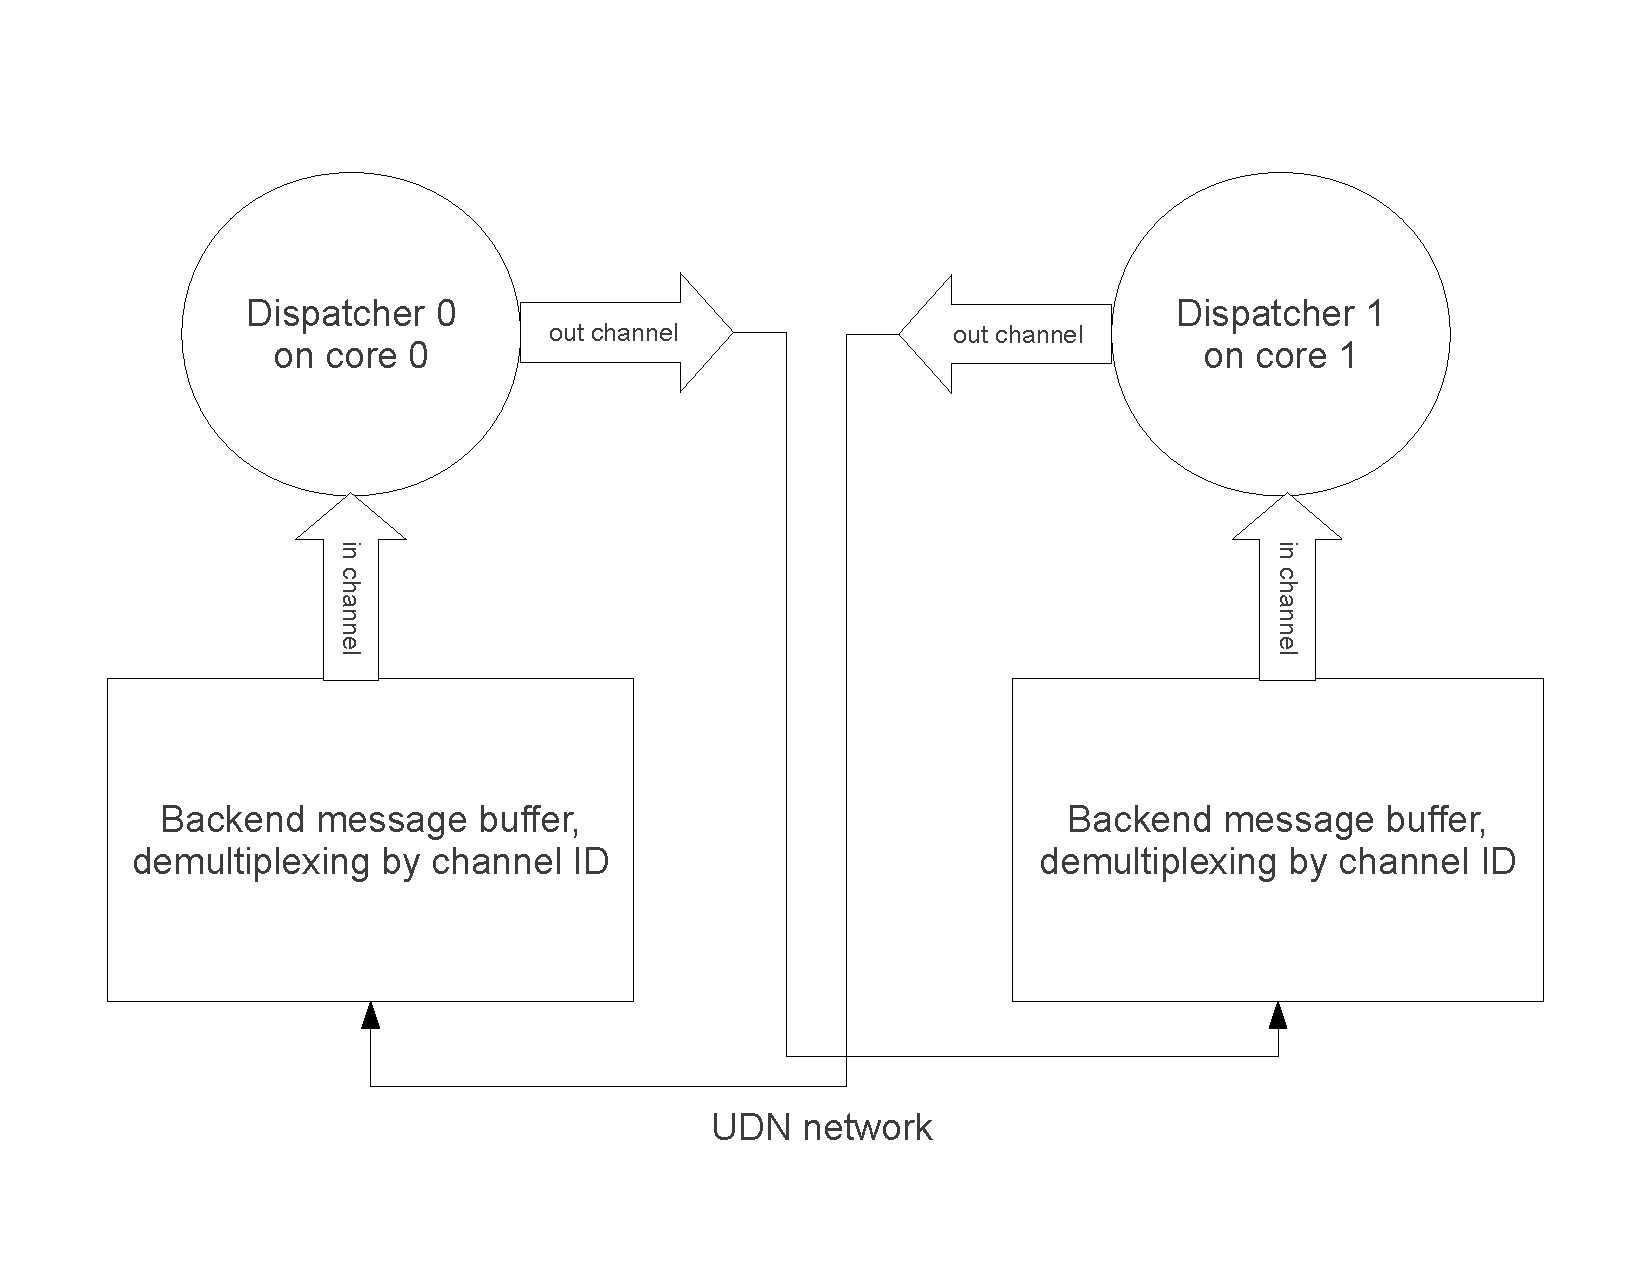
\includegraphics[scale=0.45]{figures/udn_network}
\caption{UDN backend}
\label{pic:udn}
\end{figure}

The UMP in the x86 and ARM implementations uses a polling approach to receive messages. Although the UDN network allows the use of interrupts to deliver UDN messages, we still remain the polling method, because it keeps in line with the way that messages are implemented in Barrelfish. When using messages inside the source code, the user only needs to specify if he wants to do local or remote communication. For remote communication the right backend is chosen through some compile settings, and the needed code is generated and written into some build files, so that another backend can be used by only changing the compilation option. To stay closely in the pattern we use the polling approach, so that using UDN is just a compilation option.

%*****************************************
% Results chapter 
%*****************************************

\chapter{Results}

\section{Porting Results}
By the end of this project we gained some positive outcomes. First of all we could manage to start Barrelfish on at least two cores of TilePro architecture completely and correctly. The first process \emph{init} get started, and then it calls \emph{mem{\textunderscore}serv} and \emph{monitor} to start. \emph{monitor} afterwards boots up other remaining processes on the first core, while it starts communicating with other processes via LMP. Finally \emph{spawnd} is responsible for initiating another core. Instead of booting up the second core we also could manage to run some simple user applications on the first core by combining them in the bootrom file, such as \emph{helloworld} or the console, etc.

Furthermore, the second core is completely started up. Specifically after the process \emph{monitor} on the second core gets started, it does some remote communication with the first core's \emph{monitor} at the aim of establishing a binding between dispatchers. Afterwards two dispatchers are able to send messages to each other. At this moment all communication is mainly based on our UDN network driver. By the end \emph{spawnd} is invoked, so we believe the second core now is ready according to Barrelfish team's roadmap shown in Figure \ref{pic:bootstrap}. As same as it on the first core, we also could manage to run some user applications on the second core.

\begin{figure}
\centering
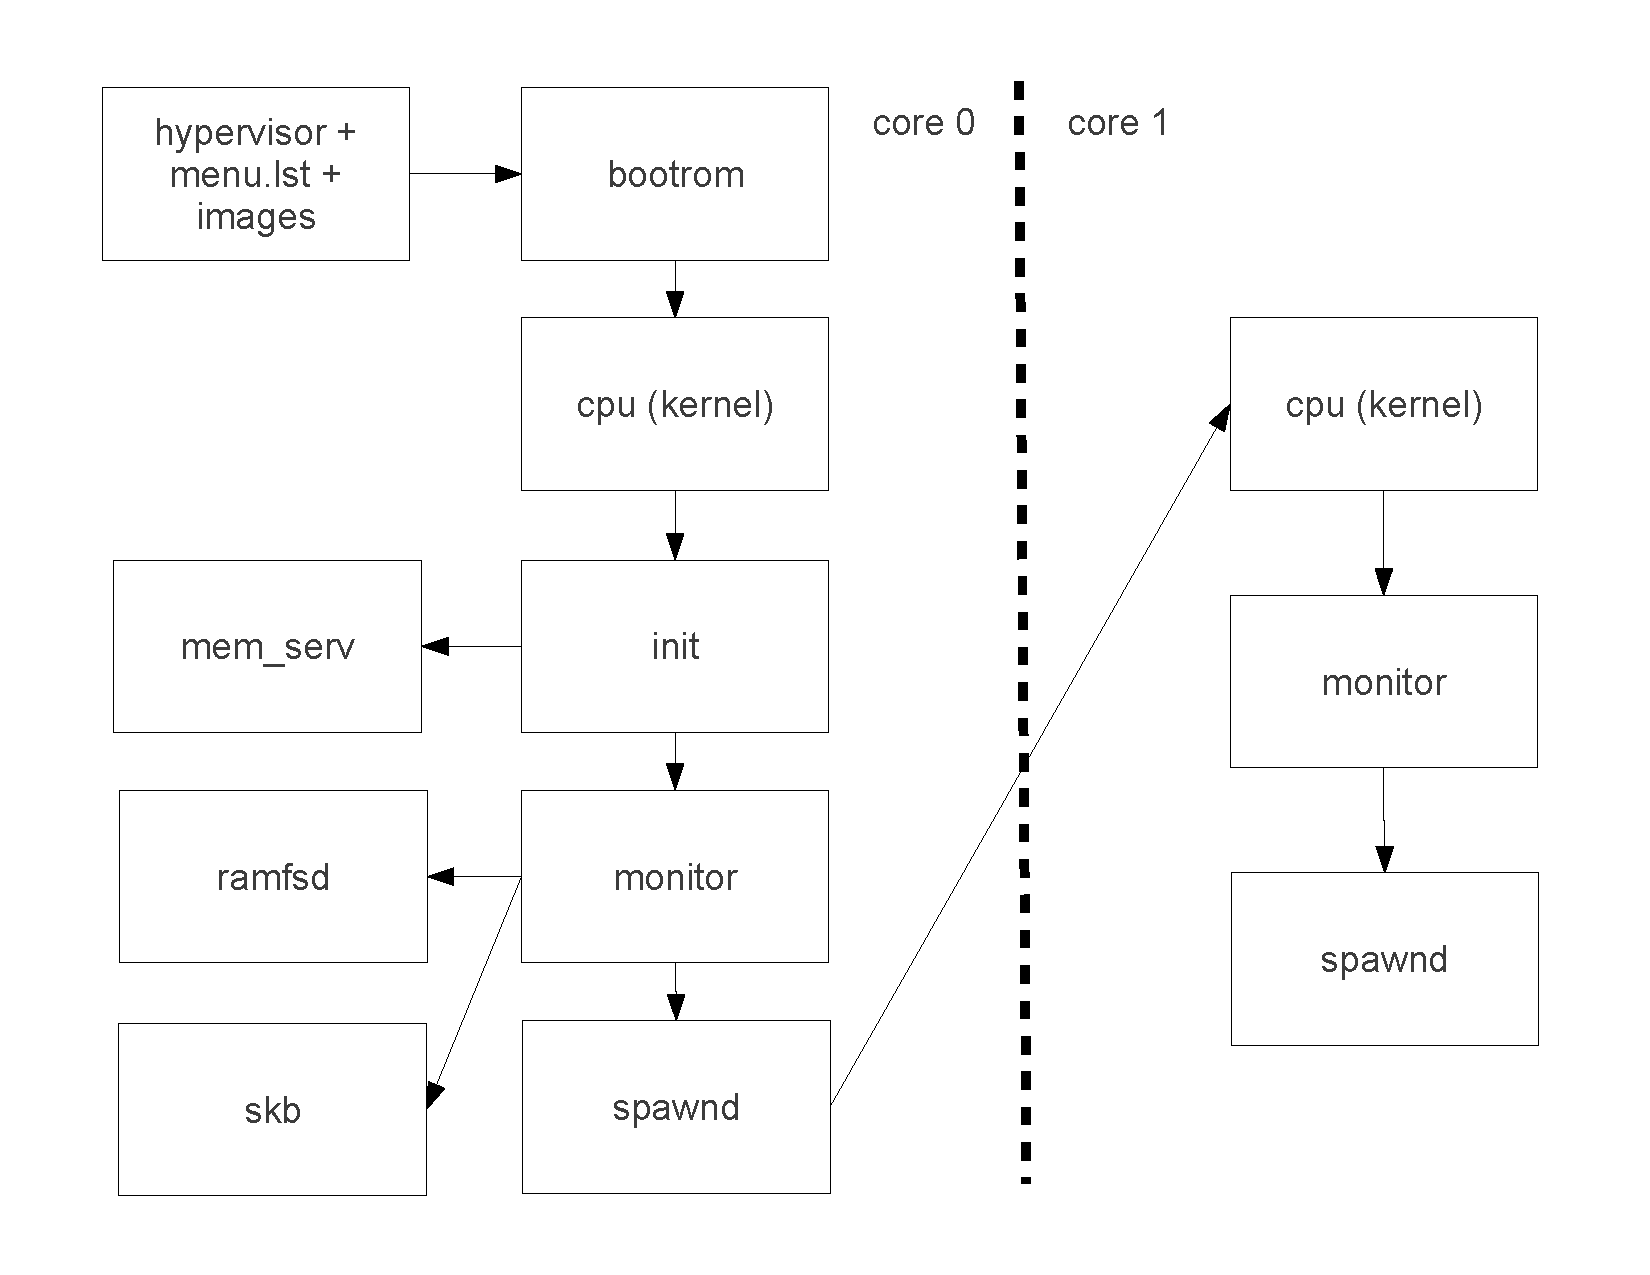
\includegraphics[scale=0.45]{figures/bootstrap_on_tilepro}
\caption{Bootstrap on TilePro}
\label{pic:bootstrap}
\end{figure}

\section{Modifications on Barrelfish}
Since normally it is not allowed to modify any setting in hardware, there is no modification on the side of TilePro. On the other hand, we add all essential architecture-related parts in Barrelfish to make sure the operating system could be run correctly.

The first step is to initiate the machine and boot up the kernel, in which includes setting up the page tables, allocating the memory, handling interrupts and system calls, and preparing for the first process to run. When the process is starting, the context switch needs to be implemented, according to TilePro's registers. In user mode, we need to implement context switch between threads in dispatcher, set up system call entry to the kernel code, high-level memory management (architecture-independent part), UDN backend and its supporting code, etc. Table \ref{table:modification} mainly summarizes the essential modules we added into Barrelfish to make it work on TilePro. 

\begin{table}[h]
\caption{Modification to Barrelfish}
\centering
\begin{tabular}{c | c} % centered columns (2 columns)
\hline \hline
Mode & Functionalities \\ [0.5ex]
\hline \hline
kernel code & boot loader, \\ 
& kernel start-up, \\
& memory allocation, \\
& page table, \\
& context switch between dispatchers, \\
& register structure for context switch, \\
& system call handler, \\
& interrupt handler \\ [0.5ex]
\hline
user code & context switch between threads, \\
& system call entry (including LMP), \\
& entry point for threads, \\
& high-level memory management (pmap), \\
& UDN backend code, \\
& UDN support code \\ [0.5ex]
\hline
\end{tabular}
\label{table:modification}
\end{table}

%*****************************************
% Conclusion chapter 
%*****************************************

\chapter{Discussion and Conclusion}
According to the bootstrap of Barrelfish we could emphasize that we succeed to port Barrelfish onto TilePro architecture, since the other cores will be using the same way to boot up as the second core, provided that there is enough memory for each core. UDN network is suggested to be exploited for the core-to-core communication, because it not only makes full use of the advantages of TilePro hardware, but also keeps in line with the design principles of Barrelfish. There is another issue we need to discuss here is the use of so-called bulk transfer technique in Barrelfish kernel. Bulk transfer is a mechanism designed to facilitate massive data exchange between processes, depending on shared memory. But this mechanism cannot be opted off, which means we have to use it anyway. That is also to say even we implement UDN network intead of UMP without any shared memory required, but at some point Barrelfish needs to call bulk transfer functionality, so the shared memory is involved more or less. TilePro actually is a shared-memory-based architecture, although it supports its own network structure to send inter-core messages. Therefore we do not need to consider more about this shared memory problem, but if someone wants to port Barrelfish onto real distributed systems without any shared memory, then a new alternative method should be invented to replace the data bulk transfer.

One of the original objectives of this project is to evaluate the efficiency of Barrelfish working on TilePro architecture after the porting, including finishing some benchmark testing work. However owing to the time limitation and the complexity of the engineer work, it is hard for us to meet all of our goals set up before. Even though we try to lead a positive start for this project to continue further in the future. At this moment what we could imagine for the future work may involve, improving the porting on the first core by starting process \emph{serial} so that the keyboard function is working, implementing a timer for the system, considering more about how to implement Barrelfish on heterogeneous systems and distributed systems, investigating more about the advantages and disadvantages of cache coherence protocols and message passing methods, establishing some benchmarks to measure Barrelfish on TilePro, etc. Therefore the future work is still tough but meaningful. Hopefully our contribution is not the end, but just the beginning.

\end{document}
